%! Author = adnansiddiquei
%! Date = 04/06/2024

\section{Results}\label{sec:results}
To assess and demonstrate the performance of our AstroCLIP model, we reproduce a subset of the downstream tasks from
the original implementation.
The models with the lowest validation loss for each embedding dimensionality (as shown in Figure~\eqref{fig:val_loss})
were selected for evaluation.
The held-out validation set (composing of 39,599 of the 197,976 image-spectra pairs) was used to evaluate the performance
by assessing the accuracy of zero-shot k-NN redshift estimations and qualitative similarity retrieval tasks.
Notation used in this section intentionally follows that of the original paper for the reader's convenience.

\subsection{Zero-shot k-NN Redshift Estimation}\label{subsec:results-redshift-regression}

\begin{figure}[t]
    \centering
    \makebox[\textwidth]{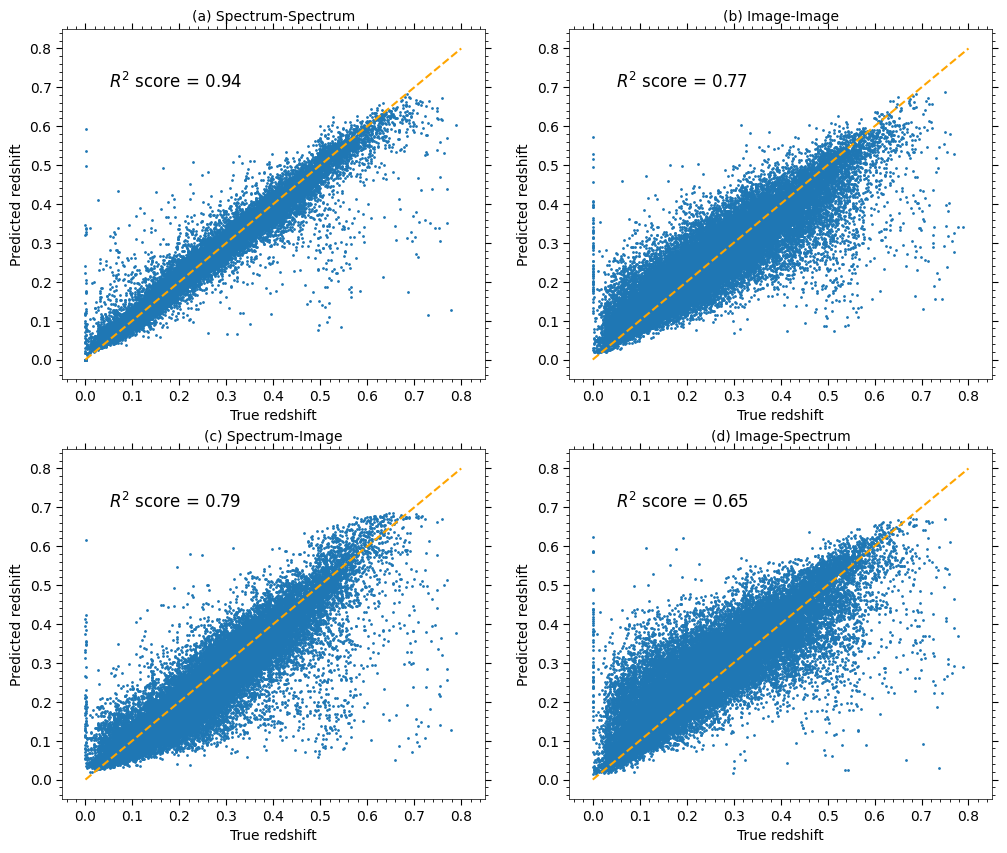
\includegraphics[width=1\textwidth]{figures/redshift_knn_regression}}
    \caption{In-modal and cross-modal zero-shot redshift predictions using k-NN regression on the learned embeddings for the
    best 128-dimensional embedding model.
    The y-axis shows the predicted redshift (the average of the 16 closest neighbours in terms of Euclidean distance) and the x-axis shows the true redshift.
    The dashed line represents a perfect prediction, and the $R^{2}$ of the fit is shown in the top left corner.
    $S_{kNN}(\mathbf{z}_{q}^{sp}, \mathbf{z}^{im})$ indicates the cross-modal prediction where a spectrums redshift was
    predicted using its 16 closes image embedded neighbours.}
    \label{fig:rkr}
\end{figure}

\begin{figure}[t]
    \centering
    \makebox[\textwidth]{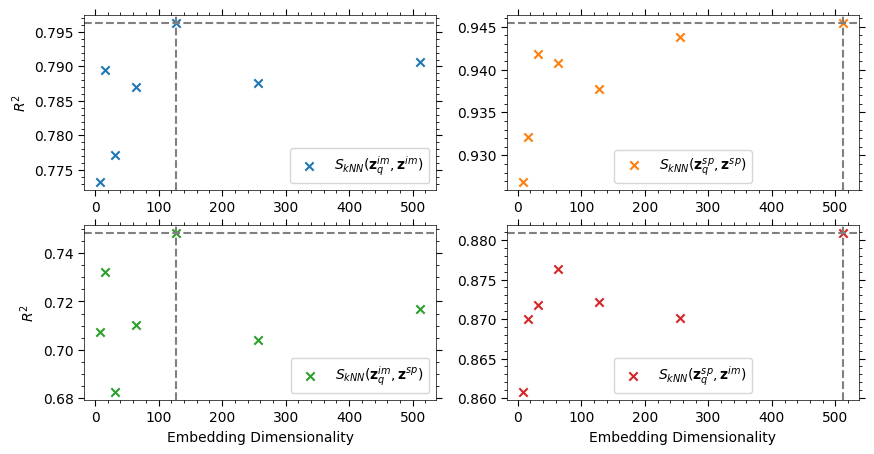
\includegraphics[width=1\textwidth]{figures/r2_vs_embedding_dim}}
    \caption{Exactly the same results as shown in Figure~\eqref{fig:rkr}, but plotted more succinctly for all embedding
    dimensionalities, and all types of in-modal and cross-modal prediction types.
    The dashed lines show the best model for each prediction type.}
    \label{fig:r2_vs_embedding_dim}
\end{figure}

Figure~\eqref{fig:rkr} shows the zero-shot redshift predictions using k-NN regression on the learned embeddings for
the best 128-dimensional embedding model.
Both in-modal (spectrum to spectrum, image to image) and both cross-modal (spectrum to image, image to spectrum)
Figure~\eqref{fig:r2_vs_embedding_dim} then shows this same data in a more succinct manner for all embedding dimensionalities.
These results demonstrate strong evidence that our AstroCLIP model is able to learn a meaningful representation of the
data, as the redshift predictions are highly correlated with the true redshift values, even with low embedding dimensionality.
For a like-by-like comparison to~\cite{astroclip} who use a 512-dimensional embedding, our photometric
$S_{kNN}(\mathbf{z}_{q}^{im}, \mathbf{z}^{im})$ redshift predictions for the 512-dimensional embedding was 0.79 which was
exactly the same as that of~\cite{astroclip}.
However, our spectroscopic $S_{kNN}(\mathbf{z}_{q}^{sp}, \mathbf{z}^{sp})$ redshift predictions for the 512-dimensional
embedding was 0.95 compared to the 0.98 reported by~\cite{astroclip}, which alludes to the effectiveness their novel
transformer architecture for spectral embeddings.
Notably, our 128-dimensional embedding model marginally outperforms the 512-dimensional embedding model in the in-modal
image to image photometric redshift prediction task with an $R^{2}$ value of 0.80, as shown on both Figure~\eqref{fig:rkr}
and Figure~\eqref{fig:r2_vs_embedding_dim}.
This indicates that the vision transformer architecture used by~\cite{astroclip} gave no significant advantage over the
2D convolutional architecture used in this work for the image embedder.
Furthermore, as shown on Figure~\eqref{fig:r2_vs_embedding_dim}, even the low 8-dimensional and 16-dimensional embedding
models perform extremely well across all prediction types, which implies that there is a meaningful amount of mutual
information between the two modalities enabling the model to learn a meaningful representation even in low dimensions.

\subsection{Retrieval by Cosine Similarity}\label{subsec:results-retrieval}
\begin{figure}[t]
    \centering
    \makebox[\textwidth]{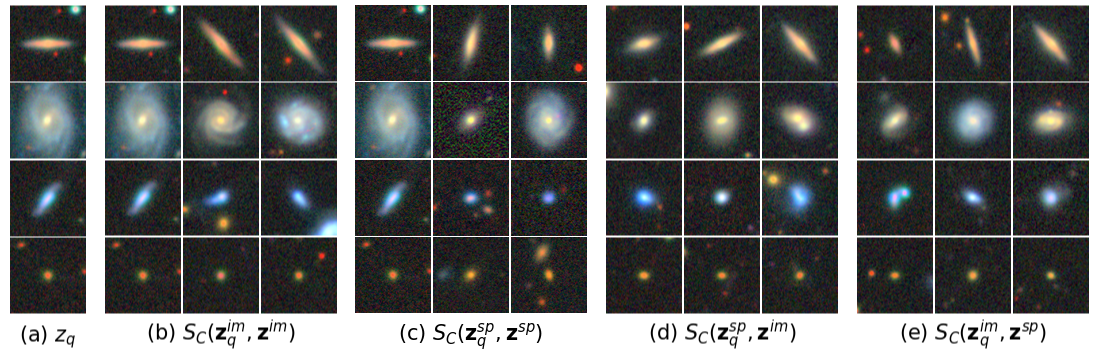
\includegraphics[width=1\textwidth]{figures/sim_search_images_all}}
    \caption{In-modal and cross-modal similarity search using cosine similarity on the learned embeddings for the
        best 128-dimensional embedding model.
        (a) shows the query galaxies; (b) shows the 3 most similar galaxies using an in-modal image to image search; and
        so on.
        By construction, the most similar in-modal galaxy to any given galaxy is itself, hence, the first column of images
        in (b) and (c) are identical to the query image in (a).}
    \label{fig:ssia}
\end{figure}

\begin{figure}[t]
    \centering
    \makebox[\textwidth]{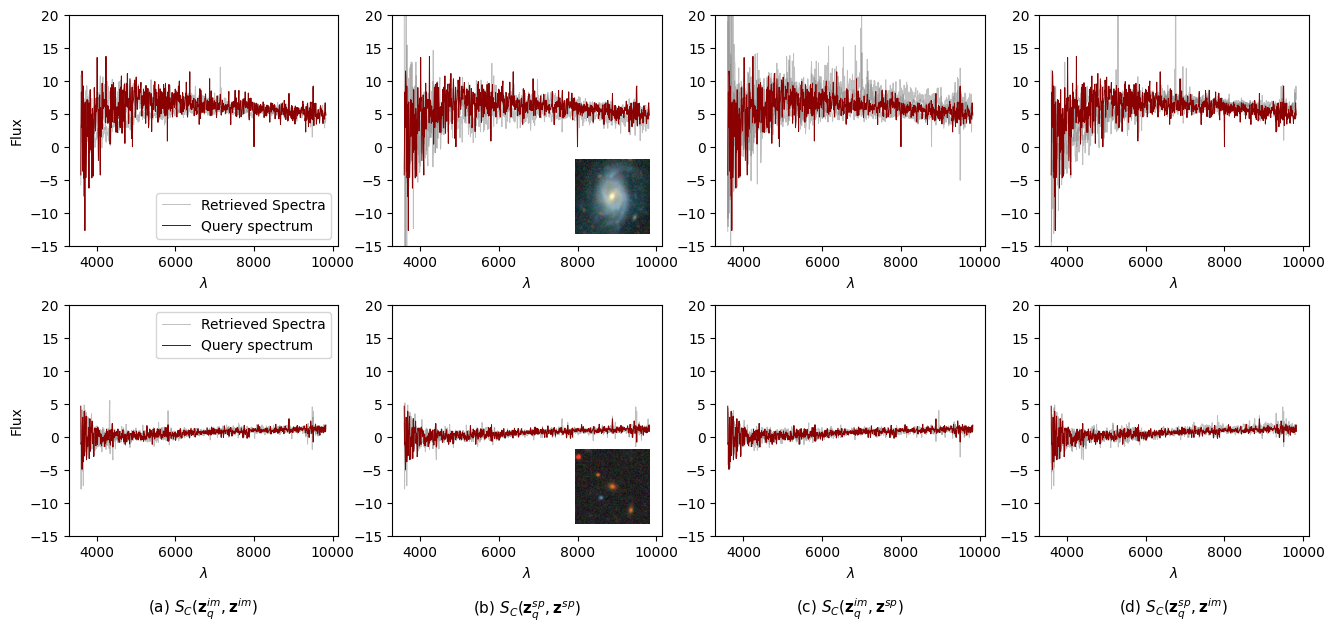
\includegraphics[width=1\textwidth]{figures/sim_search_spectra}}
    \caption{Similar to Figure~\eqref{fig:ssia}, each row in this figure depicts a single query galaxy (query spectrum in red,
        galaxy imaged in plot (b)), with each subfigure showing the spectrum of the 3 most cosine similar galaxies to the
        query galaxy by in-modal and cross-modal similarity search.}
    \label{fig:sss}
\end{figure}

The best 128-dimensional embedding model was used to perform similarity searches using cosine similarity
(Equation~\eqref{eq:cosine-similarity}) on the learned embeddings.
Unlike ~\cite{stein2021}, our model is not constrained to only performing in-modality image searches and Figures~\eqref{fig:ssia}
and~\eqref{fig:sss} show the results of both in-modal and cross-modal similarity searches for images and spectra respectively.
The results show that the model is able to retrieve similar images and spectra to the query image and spectrum, respectively,
even across modalities.
As described by ~\cite{stein2021}, this ability is critical when searching for rare astronomical sources and the cross-modal
ability of the model adds significantly to this.
